%
% File acl2015.tex
%
% Contact: car@ir.hit.edu.cn, gdzhou@suda.edu.cn
%%
%% Based on the style files for ACL-2014, which were, in turn,
%% Based on the style files for ACL-2013, which were, in turn,
%% Based on the style files for ACL-2012, which were, in turn,
%% based on the style files for ACL-2011, which were, in turn, 
%% based on the style files for ACL-2010, which were, in turn, 
%% based on the style files for ACL-IJCNLP-2009, which were, in turn,
%% based on the style files for EACL-2009 and IJCNLP-2008...

%% Based on the style files for EACL 2006 by 
%%e.agirre@ehu.es or Sergi.Balari@uab.es
%% and that of ACL 08 by Joakim Nivre and Noah Smith

\documentclass[11pt]{article}
\usepackage{acl2015}
\usepackage{times}
\usepackage{url}
\usepackage{latexsym}
\usepackage[utf8]{inputenc}
\usepackage[english]{babel}
\usepackage{graphicx}
%\setlength\titlebox{5cm}

% You can expand the titlebox if you need extra space
% to show all the authors. Please do not make the titlebox
% smaller than 5cm (the original size); we will check this
% in the camera-ready version and ask you to change it back.

\title{EE3025 IDP: Implementing Sobel Filter on Ico Board}
% \title{EE3025 IDP}

\author{Pathapati Aravind Ganesh \\
%   Affiliation / Address line 1 \\
%   Affiliation / Address line 2 \\
%   Affiliation / Address line 3 \\
  {\tt EE16BTECH11026} \\\And
  Bhavsar Jeel Alpesh\\
%   Affiliation / Address line 1 \\
%   Affiliation / Address line 2 \\
%   Affiliation / Address line 3 \\
  {\tt ES16BTECH11005} \\}

% \date{}

\begin{document}
\maketitle
% \begin{Introduction}
  
% \end{Introduction}

% \section{Credits}

% This document has been adapted from the instructions for earlier ACL
% proceedings, including those for ACL-2012 by Maggie Li and Michael
% White, those from ACL-2010 by Jing-Shing Chang and Philipp Koehn,
% those for ACL-2008 by Johanna D. Moore, Simone Teufel, James Allan,
% and Sadaoki Furui, those for ACL-2005 by Hwee Tou Ng and Kemal
% Oflazer, those for ACL-2002 by Eugene Charniak and Dekang Lin, and
% earlier ACL and EACL formats. Those versions were written by several
% people, including John Chen, Henry S. Thompson and Donald
% Walker. Additional elements were taken from the formatting
% instructions of the {\em International Joint Conference on Artificial
%   Intelligence}.

\section{Introduction}

Sobel filters are used in image processing to detect the edges of an image. We are applying a 8-bit, 3x3 sobel filter on 8-bit, 28x28 images with vertical and horizontal stride as 1 to receive a resultant 8 bit, 26x26 image.

\begin{figure}[htp]
\centering
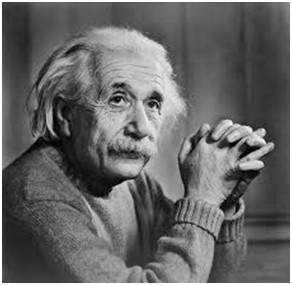
\includegraphics[width=5cm]{sobel1.jpg}
\caption{original image}
\label{fig:Einstein}
\end{figure}


\subsection{Vertical mask of Sobel operator}

When we convolve the image in 2D with the following mask, it will highlight the vertical edges of the image. 
\begin{center}
\begin{tabular}{| c| c |c |}
\hline
 1 & 0 & -1 \\ 
 \hline
 2 & 0 & -2 \\
 \hline
 1 & 0 & -1  \\
 \hline
\end{tabular}
\end{center}

The above mask calculates the difference of pixel intensities in an edge region. Since the centre column is zero, the original values of the image are not included but rather it calculates the difference of right and left pixel values around that edge. The centre values of first and third column are 2 and -2 respectively to increase the weight age to pixel values around the edge region and enhance the edge.

\begin{figure}[htp]
\centering
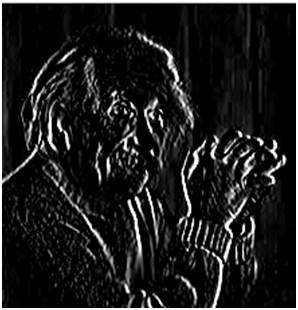
\includegraphics[width=5cm]{sobel2.jpg}
\caption{image after applying vertical mask}
\label{fig:Einstein Vertical}
\end{figure}

\subsection{Horizontal mask of Sobel operator}

When we convolve the image in 2D with the following mask, it will highlight the horizontal edges of the image. 
\begin{center}
\begin{tabular}{| c| c |c |}
\hline
 1 & 2 & 1 \\ 
 \hline
 0 & 0 & 0 \\
 \hline
 -1 & -2 & -1  \\
 \hline
\end{tabular}
\end{center}

The above mask works on the same principle as the vertical mask. Since the centre row is zero, the original values of the image are not included but rather it calculates the difference of top and bottom pixel values around that edge. The centre values of first and third row are 2 and -2 respectively to increase the weight age to pixel values around the edge region and enhance the edge.

\begin{figure}[htp]
\centering
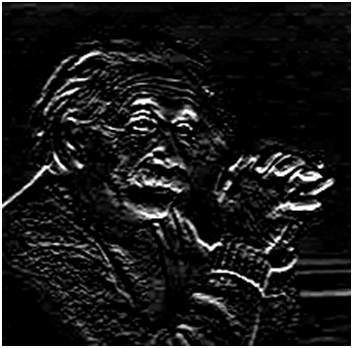
\includegraphics[width=5cm]{sobel3.jpg}
\caption{image after applying horizontal mask}
\label{fig:Einstein Vertical}
\end{figure}

\section{Implementation}
We read the image in python in image\_initialization.py and convert the pixel values into 8 bit binary format as required by verilog. The 28x28 image has 784 elements. After getting it into the correct format, the 784 values are initialized in sobel\_uart.v automatically once you run the python code. Our codes are available at \url{https://github.com/AravindGanesh/fpga_idp}. The sobel filter(vertical or horizontal) is initialized in sobel\_uart.v and the convolution takes place in conv.v. 

Run the following commands in your terminal:
\begin{quote}
\begin{verbatim}
$make initialize
$make vf_name=sobel_uart
$make receive
\end{verbatim}
\end{quote}

It performs the operation on image chosen in image\_initialization.py and saves the output image as a JPEG file.

We need to send the output 26x26 image from the icoboard back to the Raspberry Pi. The icoboard is connected to the GPIO pins so they are not accessible to us. Instead we use an FTDI to send the image back 1 pixel intensity(8 bit wide) at a time using UART protocol \url{https://github.com/ZipCPU/icozip/tree/master/rtl/uart}. Now we read the values received using receive\_img.py and save the output image on the pi.


\begin{thebibliography}{}

\bibitem[ \protect\citename{Aho and Ullman}1972]{Aho:72}
%\newblock 1972.
\newblock {\em https://www.tutorialspoint.com/dip/sobel\_operator.htm}
%\newblock Prentice-{Hall}, Englewood Cliffs, NJ.

\bibitem[ \protect\citename{Aho and Ullman}1972]{Aho:72}
%\newblock 1972.
\newblock {\em https://github.com/AravindGanesh/fpga\_idp/tree/master/src/sobel\_filter}

\bibitem[ \protect\citename{Aho and Ullman}1972]{Aho:72}
%\newblock 1972.
\newblock {\em https://github.com/ZipCPU/icozip/tree/master/rtl/uart}

\end{thebibliography}

\end{document}